\documentclass[notes,11pt, aspectratio=169]{beamer}

\usepackage[brazilian]{babel}
\usepackage[utf8]{inputenc}
\usepackage[T1]{fontenc}

\usepackage[numbers]{natbib}

\newcommand{\citeonline}[1]{
    % \bibliographystyle{sbc}
    \bibliographystyle{abbrvnat}
    \setcitestyle{authoryear,open={(},close={)}}
    \cite{#1}
}

\usepackage{pgfpages}
% These slides also contain speaker notes. You can print just the slides,
% just the notes, or both, depending on the setting below. Comment out the want
% you want.
\setbeameroption{hide notes} % Only slide
%\setbeameroption{show only notes} % Only notes
%\setbeameroption{show notes on second screen=right} % Both

\usepackage{helvet}
\usepackage[default]{lato}
\usepackage{array}
\usepackage{tikz}
\usepackage{verbatim}
\setbeamertemplate{note page}{\pagecolor{yellow!5}\insertnote}
\usetikzlibrary{positioning}
\usetikzlibrary{snakes}
\usetikzlibrary{calc}
\usetikzlibrary{arrows}
\usetikzlibrary{decorations.markings}
\usetikzlibrary{shapes.misc}
\usetikzlibrary{matrix,shapes,arrows,fit,tikzmark}
\usepackage{amsmath}
\usepackage{mathpazo}
\usepackage{hyperref}
\usepackage{lipsum}
\usepackage{multimedia}
\usepackage{multirow}
\usepackage{graphicx}
\usepackage{dcolumn}
\usepackage{bbm}
\newcolumntype{d}[0]{D{.}{.}{5}}

\usepackage{changepage}
\usepackage{appendixnumberbeamer}
\newcommand{\beginbackup}{
   \newcounter{framenumbervorappendix}
   \setcounter{framenumbervorappendix}{\value{framenumber}}
   \setbeamertemplate{footline}
   {
     \leavevmode%
     \hline
     box{%
       \begin{beamercolorbox}[wd=\paperwidth,ht=2.25ex,dp=1ex,right]{footlinecolor}%
%         \insertframenumber  \hspace*{2ex} 
       \end{beamercolorbox}}%
     \vskip0pt%
   }
 }
\newcommand{\backupend}{
   \addtocounter{framenumbervorappendix}{-\value{framenumber}}
   \addtocounter{framenumber}{\value{framenumbervorappendix}} 
}

\usepackage[space]{grffile}
\usepackage{booktabs}

% These are my colors -- there are many like them, but these ones are mine.
\definecolor{blue}{RGB}{0,114,178}
\definecolor{red}{RGB}{213,94,0}
\definecolor{yellow}{RGB}{240,228,66}
\definecolor{green}{RGB}{0,158,115}

\hypersetup{
  colorlinks=false,
  linkbordercolor = {white},
  linkcolor = {blue}
}


%% I use a beige off white for my background
\definecolor{MyBackground}{RGB}{255,253,218}

%% Uncomment this if you want to change the background color to something else
%\setbeamercolor{background canvas}{bg=MyBackground}

%% Change the bg color to adjust your transition slide background color!
\newenvironment{transitionframe}{
  \setbeamercolor{background canvas}{bg=yellow}
  \begin{frame}}{
    \end{frame}
}

\setbeamercolor{frametitle}{fg=blue}
\setbeamercolor{title}{fg=black}
\setbeamertemplate{footline}[frame number]
\setbeamertemplate{navigation symbols}{} 
\setbeamertemplate{itemize items}{-}
\setbeamercolor{itemize item}{fg=blue}
\setbeamercolor{itemize subitem}{fg=blue}
\setbeamercolor{enumerate item}{fg=blue}
\setbeamercolor{enumerate subitem}{fg=blue}
\setbeamercolor{button}{bg=MyBackground,fg=blue,}



% If you like road maps, rather than having clutter at the top, have a roadmap show up at the end of each section 
% (and after your introduction)
% Uncomment this is if you want the roadmap!
% \AtBeginSection[]
% {
%     \begin{frame}
%         \frametitle{Roteiro}
%         \tableofcontents[currentsection]
%     \end{frame}
% }
\setbeamercolor{section in toc}{fg=blue}
\setbeamercolor{subsection in toc}{fg=red}
\setbeamersize{text margin left=1em,text margin right=1em} 

\newenvironment{wideitemize}{\itemize\addtolength{\itemsep}{10pt}}{\enditemize}

\title[]{\textcolor{blue}{Classificação de emoções por meio de expressões faciais em sala de aula
}}
\author[PGP]{}
\institute[UTFPR]{\small{\begin{tabular}{c}
Marcus V. S. Maziero; Paulo R. K. Nakaima; Vitor Hugo Borges Basseto\\
\\
\multicolumn{1}{c}{Cornélio Procópio UTFPR} \\
\end{tabular}}}

\date{\today}


%%% TIKZ STUFF
\tikzset{   
        every picture/.style={remember picture,baseline},
        every node/.style={anchor=base,align=center,outer sep=1.5pt},
        every path/.style={thick},
        }
\newcommand\marktopleft[1]{%
    \tikz[overlay,remember picture] 
        \node (marker-#1-a) at (-.3em,.3em) {};%
}
\newcommand\markbottomright[2]{%
    \tikz[overlay,remember picture] 
        \node (marker-#1-b) at (0em,0em) {};%
}
\tikzstyle{every picture}+=[remember picture] 
\tikzstyle{mybox} =[draw=black, very thick, rectangle, inner sep=10pt, inner ysep=20pt]
\tikzstyle{fancytitle} =[draw=black,fill=red, text=white]
%%%% END TIKZ STUFF

\begin{document}

% Title Slide
\begin{frame}
\maketitle

\end{frame}

% ROTEIRO
\begin{frame}
    \frametitle{Roteiro}
    \tableofcontents
\end{frame}


% INTRO
\section{Introdução}
\begin{transitionframe}
  \begin{center}
    { \Huge \textcolor{black}{Introdução}}
  \end{center}
\end{transitionframe}

% CONTEXTO
\section{Contexto}
\begin{transitionframe}
  \begin{center}
    { \Huge \textcolor{black}{Contexto}}
  \end{center}
\end{transitionframe}

\begin{frame}{Blockchain e propriedades não funcionais}
\begin{columns}[T] % align columns
	\begin{column}{.58\textwidth}
		\resizebox{\textwidth}{!}{
			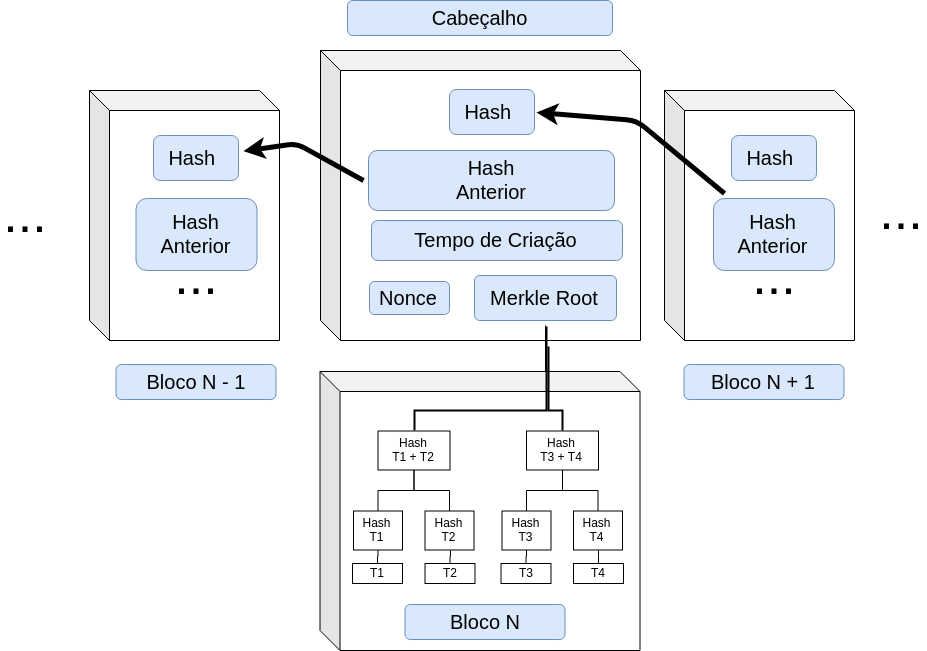
\includegraphics{fig/bc-esquematizada.png}
		}
	\end{column}%
	\hfill%
	\begin{column}{.38\textwidth}
		\begin{wideitemize}
			\item Integridade
			\item Imutabilidade
			\item Irretratabilidade
			\item Transparência
			\item Desintermediação
		\end{wideitemize}
	\end{column}%
\end{columns}
\footnote{Fonte: Adaptado de teste}
\end{frame}

% PROBLEMA
\section{Problema}
\begin{transitionframe}
  \begin{center}
    { \Huge \textcolor{black}{Problema}}
  \end{center}
\end{transitionframe}


% OBJETIVOS
\section{Objetivo}
\begin{transitionframe}
  \begin{center}
    { \Huge \textcolor{black}{Objetivo}}
  \end{center}
\end{transitionframe}

% TRABALHOS RELACIONADOS
\section{Trabalhos Relacionados}
\begin{transitionframe}
  \begin{center}
    { \Huge \textcolor{black}{Trabalhos Relacionados}}
  \end{center}
\end{transitionframe}


% METODOLOGIA
\section{Metodologia}
\begin{transitionframe}
  \begin{center}
    { \Huge \textcolor{black}{Metodologia}}
  \end{center}
\end{transitionframe}

\begin{frame}{Ambiente de Software}
\begin{columns}[T] % align columns
	\begin{column}{.38\textwidth}
		\begin{wideitemize}
			\item Várias \textcolor{red}{dependências}
			\item Diferentes \textcolor{red}{versões}
			\item Permissão de usuário
			\item Fonte: \emph{\textcolor{blue}{\href{https://medium.com/haloblock/how-to-use-oyente-a-smart-contract-security-analyzer-solidity-tutorial-86671be93c4b}{Tutorial}}}
			e
			\emph{\textcolor{blue}{\href{https://github.com/melonproject/oyente}{GitHub}}}
		\end{wideitemize}
	\end{column}%
	\hfill%
	\begin{column}{.58\textwidth}
		\makebox[\linewidth][c]{
			\resizebox{\linewidth}{!}{
				
\includegraphics{./fig/py2orpy3.jpg}
			}
		}
	\end{column}%
\end{columns}
\end{frame}


% RESULTADOS
\section{Resultados}
\begin{transitionframe}
  \begin{center}
    { \Huge \textcolor{black}{Resultados}}
  \end{center}
\end{transitionframe}

\begin{frame}{Resulados}
\begin{columns}[T] % align columns
	\begin{column}{.38\textwidth}
		\begin{wideitemize}
			\item Evitar \textcolor{red}{superestimação} dos resultados
			\item Melhores combinações de \textcolor{blue}{normalização}, \textcolor{blue}{número de características}
		\end{wideitemize}
	\end{column}%
	\hfill%
	\begin{column}{.58\textwidth}
		\makebox[\linewidth][c]{
			\resizebox{\linewidth}{!}{
				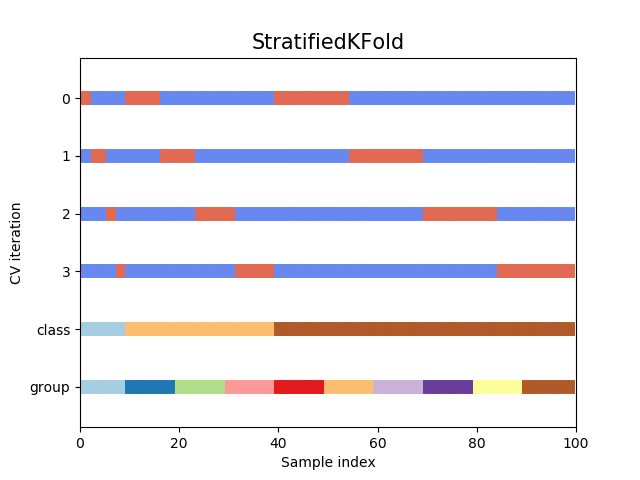
\includegraphics{./fig/strat_kfold.png}
			}
		}
	\end{column}%
\end{columns}
\end{frame}

\begin{frame}{Decritor LBP - Acurácia -10-fold}
\begin{center}
	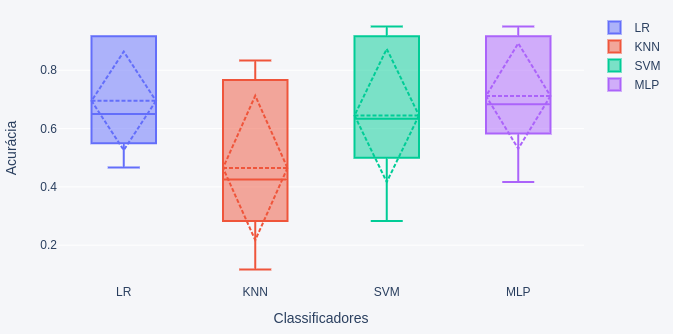
\includegraphics[width=.8\textwidth,height=.7\textheight]{./fig/box_result_lbp.png}
\end{center}
Fonte: \emph{\textcolor{blue}{\href{https://colab.research.google.com/drive/15Ozutw22u9wfAXisgqfhmA33P3s0fbWp?usp=sharing}{Colab}}}
e
\emph{\textcolor{blue}{\href{https://github.com/guimpo/hand_on_again_ai_master/}{GitHub}}}
\end{frame}

\begin{frame}{Decritor Gabor - Acurácia - 10-fold}
\begin{center}
	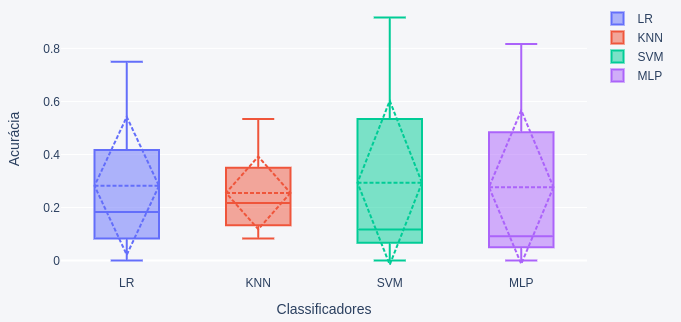
\includegraphics[width=.8\textwidth,height=.7\textheight]{./fig/box_result_gabor.png}
\end{center}
Fonte: \emph{\textcolor{blue}{\href{https://colab.research.google.com/drive/1U0qTE3tIe4U-ODfb8-bq7YlJft0raeHX?usp=sharing}{Colab}}}
e
\emph{\textcolor{blue}{\href{https://github.com/guimpo/hand_on_again_ai_master/}{GitHub}}}
\end{frame}

% CONCLUSÃO
\section{Conclusão e Trabalhos Futuros}
\begin{transitionframe}
  \begin{center}
    { \Huge \textcolor{black}{Conclusão e Trabalhos Futuros}}
  \end{center}
\end{transitionframe}

\begin{frame}{Conclusão}
\begin{wideitemize}
	\item Use the \texttt{\textbackslash appendix} command to restart the numbering
	\item The frame counter says this is the last slide, but it's not
	\item (Test it, see you on next page)
\end{wideitemize}
\end{frame}

\begin{frame}{Trabalhos Futuros}
\begin{wideitemize}
	\item Utilizar outras bases de imagens
	\item Aplicar detecção facial nas imagens
	\item Encontrar os melhores parãmetros para os classificadores
	\item Utilizar \textit{Deep Learning}
\end{wideitemize}
\end{frame}

\section{Referências}
{
\begin{frame}{Referências}
\bibliography{references}
\end{frame}
}


\begin{transitionframe}
  \begin{center}
    \Huge Apêndice
  \end{center}
\end{transitionframe}


\appendix
\begin{frame}{Docker}
\begin{center}
	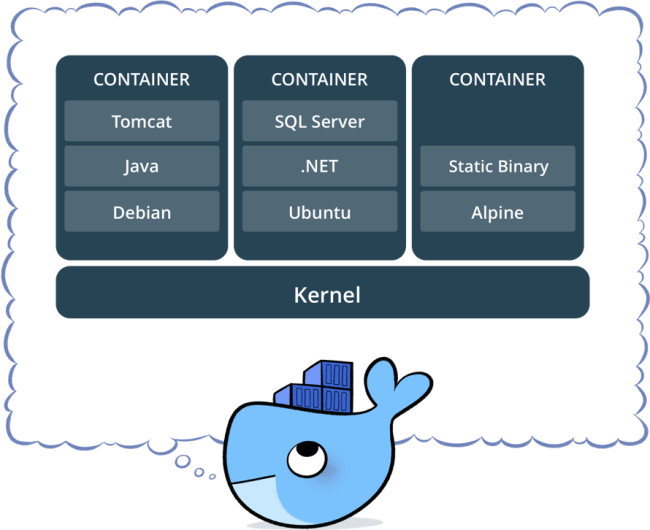
\includegraphics[width=.6\textwidth,height=.9\textheight]{./fig/docker1.png}
\end{center}
\end{frame}


\begin{frame}{Catálogo de fraquezas em Contratos Inteligentes}
\makebox[\linewidth][c]{
\resizebox{.6\linewidth}{!}{
	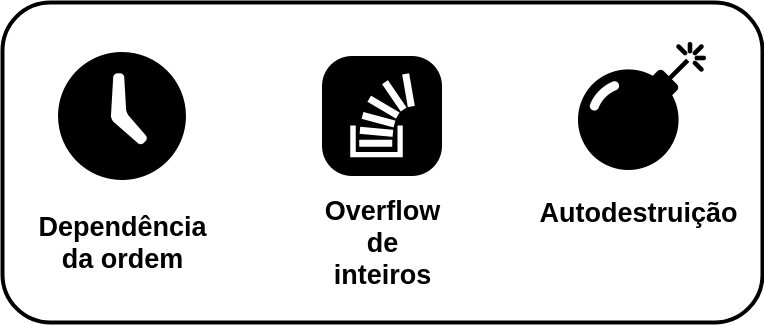
\includegraphics{./fig/fraquezas.png}
}
}

\hfill%
\begin{wideitemize}
\item Fonte: \emph{\textcolor{blue}{\href{https://swcregistry.io/docs/SWC-106}{Cátalogo}}}
e
\emph{\textcolor{blue}{\href{https://github.com/SmartContractSecurity/SWC-registry}{GitHub}}}
\item Aprendizado, divulgação, testes \cite{knuth:84} \cite{boulic:91} \citeonline{smith:99}
\end{wideitemize}
\end{frame}


\begin{frame}{Almost done!}
  \begin{wideitemize}
  \item Use the \texttt{\textbackslash appendix} command to restart the numbering
  \item The frame counter says this is the last slide, but it's not
  \item (Test it, see you on next page)
  \end{wideitemize}
\end{frame}

\end{document}
